\documentclass[12pt]{article}

\addtolength{\textwidth}{.8in}
\addtolength{\hoffset}{-.4in}
\addtolength{\textheight}{1in}
\addtolength{\voffset}{-1in}

\usepackage{amsmath}
\usepackage{graphicx}
\usepackage{amsfonts}
\usepackage{paralist}
\usepackage{fancyvrb}
\usepackage{textcomp} % to convert funny quotes to straight quotes
\setlength{\parindent}{15pt}

\renewcommand*{\thefootnote}{\fnsymbol{footnote}}

\begin{document}

\begin{center}
\begin{Large}
DATA 219 Notes -- Jan. 30, 2018
\end{Large}
\end{center}

\section{Generating synthetic data sets, cont.}

\subsection{Numerical data, cont.}

Last time we generated synthetic pairs of numerical vectors which were
partially, but not completely, correlated. Our idea for this was to (1)
generate the first vector of values randomly, (2) multiply that first vector
times some factor to transform it to the different scale required by the
second vector, and (3) add some random noise. Our canonical example was this:

\begin{Verbatim}[fontsize=\footnotesize,samepage=true]
sat_scores = np.random.normal(1400, 350, 100)
gpas = sat_scores * (2.5 / 1400) + np.random.normal(0, 1, 100)
\end{Verbatim}

This is a good first attempt. Notice two assumptions/limitations, though:

\begin{enumerate}
\item We're assuming that the relationship between the two variables is
\textit{linear} --- namely, that ``the first value times a constant" is a good
estimate for the second value. In reality, of course, the relationship is
often more complex: it might be better modeled as the \textit{square} of the
first value, for instance, or ``$e$ to the" first value, or the cube root of
the first value, \textit{etc.}
\item We're assuming that the ``zero point" for the two variables coincide:
in other words, a zero for one value would on average roughly correspond to a
zero for the other. In the above case, we're assuming that a person who got a
0 on the SAT would have, on average, a 0 GPA. If this isn't appropriate, we
should add an \textbf{intercept term} (a constant) to our generative formula.
This takes our generated second variable and just shifts it, wholesale, to a
new region of the number range.
\end{enumerate}

By the way, how do we go about estimating the numbers for these things,
anyway? If we include an intercept, our formula for generating the second
value boils down to:

\begin{center}
\texttt{second\_value} = $\alpha \cdot$ \texttt{first\_value}
+ $\beta$ + \texttt{np.random.normal(0, $\sigma$, $n$)}
\end{center}

and we have to figure out values for $\alpha$, $\beta$, and $\sigma$.

\vspace{.1in}
My approach: identify a ``high-ish" value of the first variable, and estimate
the roughly-on-average corresponding value of the second variable. Then do the
same for a ``low-ish" value. Then, plug those into the familiar $y=mx+b$
formula (or, in our case, $y=\alpha x + \beta$) you learned in middle school
and solve for the slope and intercept.

\subsubsection{Example}

I'm going to generate a synthetic data set of two variables: the number of
hours a person has practiced playing the Dance Dance Revolution (DDR)
videogame in their lifetime, and the score they achieved in a DDR contest (on
the song \textit{Kakumei}). Clearly, there should be some (positive)
relationship between the two quantities: when \texttt{num\_hrs} is high, you'd
expect \texttt{score} to also be high. If you're familiar with the game,
though, you know that the zero points for these variables do \textit{not}
coincide: if you've never ever played at all, you'll still manage to stumble
through the song, learn how to play as you go, and get a positive score.

Let's generate the \texttt{num\_hrs} variable first, and then generate the
\texttt{score} variable based on that.

Based on my knowledge of the game, I estimate:
\begin{compactitem}
\item A good-ish player who has practiced for 100 hours might get a score of
around 60,000,000.
\item A sucky-ish player who has practiced for only 10 hours might get a score
of around 30,000,000.
\end{compactitem}

Running the algebra, I get:
\begin{align*}
60,000,000 &= \alpha \cdot 100 + \beta\\
30,000,000 &= \alpha \cdot 10 + \beta\\
\end{align*}
\vspace{-.7in}
\begin{center}
\dots \textit{insert algebra here} \dots \\
$\alpha = 333,333, \beta = 26,666,666$
\end{center}

Thus we get back-of-the-envelope estimates of $\alpha$ and $\beta$.

How to estimate $\sigma$? Play with it. If you're using the normal
distribution, remember that two-thirds of your data points will fall between
one standard deviation from the mean. I think two-thirds of my 100-hour
practicers might get between 50,000,000 and 70,000,000. So I'll go with a
$\sigma$ of 10,000,000 and see how that looks. My final code for a synthetic
data set of 200 players is:

\begin{Verbatim}[fontsize=\footnotesize,samepage=true]
num_hrs = np.random.normal(50,20,200).clip(0,100)
score = num_hrs * 333333 + 26666666 + np.random.normal(0,10000000,200)
\end{Verbatim}

(The ``\texttt{.clip()}" makes sure all the \texttt{num\_hrs} values are
between 0 and 100.)

This looks pretty decent:

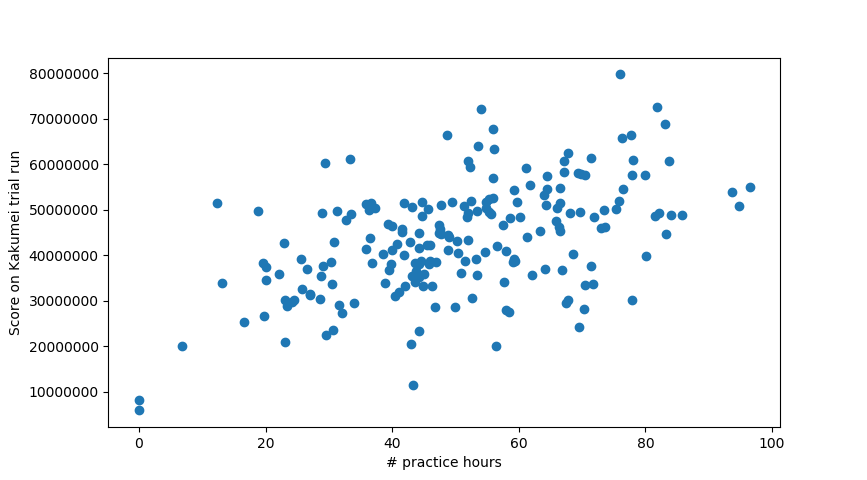
\includegraphics[width=0.9\textwidth]{ddr.png}

Note: there's also a \texttt{multivariate\_normal} function in the
\texttt{scipy.stats} package which can generate these kinds of correlated data
sets more powerfully.

\subsection{Synthetic categorical data}

So that's numeric, now what about categorical data?

\subsubsection{Uncorrelated categorical variables}

Let's generate a data set with 2000 registered voters in Fredericksburg, 54\%
Democrats and 46\% Republicans. We'll also generate their pick for the
Superbowl: Eagles (30\%) or Patriots (70\%).

Since these variables are uncorrelated, we generate each one separately. To
keep this section consistent with those following, I'm going to make the
\texttt{party} variable very regular: all the Democrats in a row, followed by
all the Republicans in a row. The \texttt{np.repeat()} function is useful
here.

\begin{Verbatim}[fontsize=\footnotesize,samepage=true]
party = np.append(np.repeat('Democrat',.54*2000),np.repeat('Republican',.46*2000))
superbowl = np.random.choice(['Eagles','Patriots'], p=[.3,.7], size=2000)
\end{Verbatim}

As expected, a $\chi^2$ test's p-value shows no correlation:

\begin{Verbatim}[fontsize=\footnotesize,samepage=true]
>>> pd.crosstab(superbowl,party)
          Democrat  Republican
Eagles         334         286
Patriots       746         634

>>> round(scipy.stats.chi2_contingency(pd.crosstab(superbowl,party))[1],2)
0.98
\end{Verbatim}

\subsubsection{Completely correlated categorical variables}

Now let's add a ``\texttt{party\_color}" categorical variable that gives the
associated color of each voter's political party (blue for Democrats and red
for Republicans). Since this is perfectly correlated with \texttt{party}, we
can generate another vector from scratch with the same setup. The
\texttt{np.where()} function comes in handy:

\begin{Verbatim}[fontsize=\footnotesize,samepage=true]
party_color = np.where(party=='Democrat','blue','red')
\end{Verbatim}

\texttt{np.where()} is tricky but powerful. It takes three arguments -- a
vector of booleans (\texttt{true}s and \texttt{false}s), and two other
arguments which are used as substitutions. It produces a vector \textit{that
includes the second argument in every position where the first is
\texttt{true}, and the third argument everywhere it's \texttt{false}.} In the
current example, we're saying ``for every place that the \texttt{party} vector
has a \texttt{\textquotesingle Democrat\textquotesingle } value, put
\texttt{\textquotesingle blue\textquotesingle } in this new vector you're
making for me, and put \texttt{\textquotesingle red\textquotesingle } everywhere else."

We thus (obviously) get perfect correlation:

\begin{Verbatim}[fontsize=\footnotesize,samepage=true]
In [30]: pd.crosstab(party,party_color)
Out[30]: 
            blue  red
Democrat    1080    0
Republican     0  920

>>> round(scipy.stats.chi2_contingency(pd.crosstab(party, party_color))[1],2)
0.0
\end{Verbatim}

\subsubsection{Somewhat correlated categorical variables}

Finally, let's create a ``\texttt{gun\_owner}" categorical variable which has
the value \texttt{True} or \texttt{False} for each voter: it should be true
for roughly 44\% of Republicans and for 20\% of Democrats. For this, we can go
back to our friend \texttt{np.where()}:

\begin{Verbatim}[fontsize=\footnotesize,samepage=true]
gun_owner = np.where(party=='Democrat',
    np.random.choice([True,False],p=[.2,.8],size=2000),
    np.random.choice([True,False],p=[.44,.56],size=2000))
\end{Verbatim}

This time, our second and third arguments to \texttt{np.where()} are
\textit{vectors themselves}. We're saying, ``in every position where
\texttt{party} has a \texttt{\textquotesingle Democrat\textquotesingle }, use the corresponding value from our
random vector that is 80\% \texttt{false}s. Otherwise, use the corresponding
value from a different random vector that is 56\% \texttt{false}s."

Checking, we do get the desired correlation:

\begin{Verbatim}[fontsize=\footnotesize,samepage=true]
>> pd.crosstab(party,gun_owner)
            False  True 
Democrat      841    239
Republican    505    415

>> scipy.stats.chi2_contingency(pd.crosstab(party,gun_owner))[1]
1.5994151557508934e-27
\end{Verbatim}

\section{Kernel Density Estimates (KDEs)}

\subsection{Limitations of histograms}

Histograms are a great tool for seeing the distribution of a numerical,
univariate sample. One problem with them, though, is that a data set doesn't
uniquely determine a histogram: instead, we must specify parameters such as
the bin size and the ``alignment" of the bins (\textit{i.e.}, where exactly
the breaks occur), and the resulting display is colored by those choices.

Consider this simple data set (from Janert, 2010):

\begin{center}
\texttt{2.1, 2.3, 1.9, 1.8, 1.4, 2.6, 1.7, 2.2}
\end{center}

Suppose we choose a bin width of 1. If we positioned the \textit{left} edge of
each bin at 0, 1, 2, 3, ..., we would get this histogram:

\begin{Verbatim}[fontsize=\footnotesize,samepage=true]
data = np.array([2.1, 2.3, 1.9, 1.8, 1.4, 2.6, 1.7, 2.2])
plt.hist(data, bins=[0,1,2,3,4])
\end{Verbatim}

\begin{center}
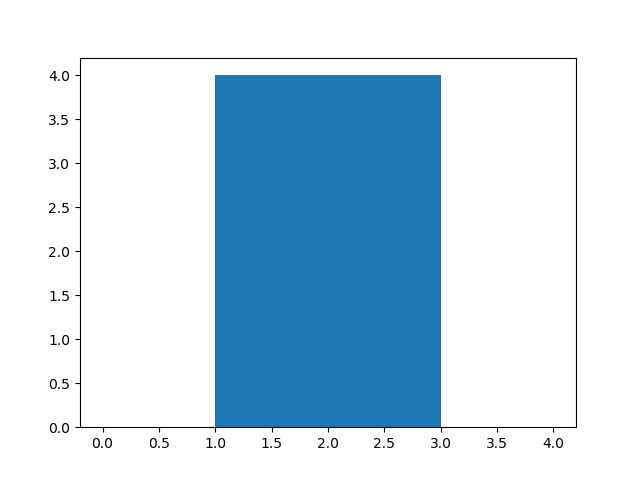
\includegraphics[width=0.7\textwidth]{hist1.png}
\end{center}

Our interpretation would probably be: ``looks like the values occur pretty
uniformly throughout the range 1-3." But if we shifted our bin alignment to be
on the ``halves" (0.5, 1.5, 2.5, ...), we get this:

\begin{Verbatim}[fontsize=\footnotesize,samepage=true]
plt.hist(data, bins=[-.5,0.5,1.5,2.5,3.5,4.5])
\end{Verbatim}

\begin{center}
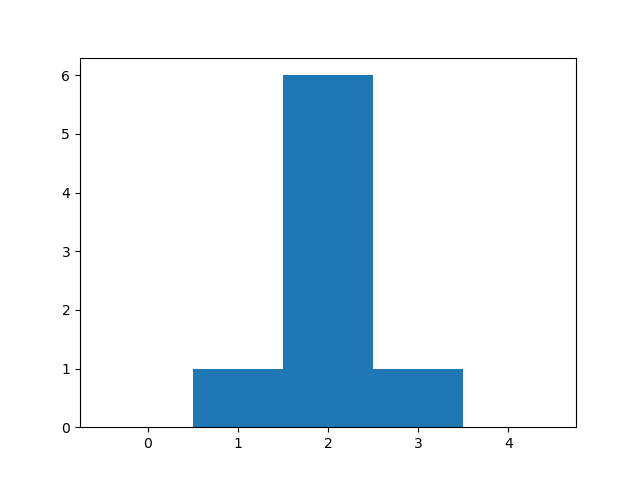
\includegraphics[width=0.8\textwidth]{hist2.png}
\end{center}

Now we may be liable to think: ``it looks like a steeply-peaked distribution
with most values right near the center value of 2."

\vspace{.2in}
Yet the data is the same!
\vspace{.2in}

Histograms have a couple other problems as well:

\begin{itemize}
\itemsep.1em
\item They inherently lose information, since by definition data points with
specific, precise values are munged into ``the nearest bin."
\item They don't handle outliers very well. A single outlier way outside the
normal range forces us to either (a) include a lot of empty cells in the
middle, or (b) choose an unreasonably wide bin width that doesn't work for the
majority of points.
\end{itemize}

One solution to these problems is a more advanced technique called
\textit{Kernel Density Estimates.}

\subsection{Kernels}

A ``kernel" is defined as a single, strongly-peaked function that has an area
under its curve of exactly 1. Normally (no pun intended!) we will use a
\textit{Gaussian kernel}, which means ``a bell curve a la the normal
distribution." 

One thing we have to decide is the \textit{width} of this kernel --- which in
our case essentially means ``the standard deviation of the normal
distribution we're using." This is kind of like having to choose the bin width
for histograms, but in practice it turns out not to 

To form a KDE, we place a ``copy" of this kernel at each data point, and then
add up all the kernel contributions to make a smooth curve.

There are several different ways to do this with Python packages. The Seaborn
library has a good ``\texttt{kdeplot()}" function. Using straight SciPy, we
can call the \texttt{gaussian\_kde()} function and pass it the bandwidth as a
second argument. This returns a function that can be used to evaluate the KDE
at any data point. (Read that sentence again: a function that returns a
function? It can be confusing.) Then, we can plot it by creating a range of
values to evaluate the KDE at, and plotting those values against the KDE's
values.

It's easier than it sounds when you run the actual code:

\begin{Verbatim}[fontsize=\footnotesize,samepage=true]
import scipy.stats
kde = scipy.stats.gaussian_kde(data,bw_method=2)
x_vals = np.arange(0,4,.1)
plt.plot(x_vals,kde(x_vals))
\end{Verbatim}

Choosing a larger kernel width effectively smooths out the KDE more, making
each point ``fuzzier" with respect to its actual position. Choosing a narrower
kernel width focuses each data point's contribution more at its actual value,
which makes the plot choppier.

\begin{figure}
\centering
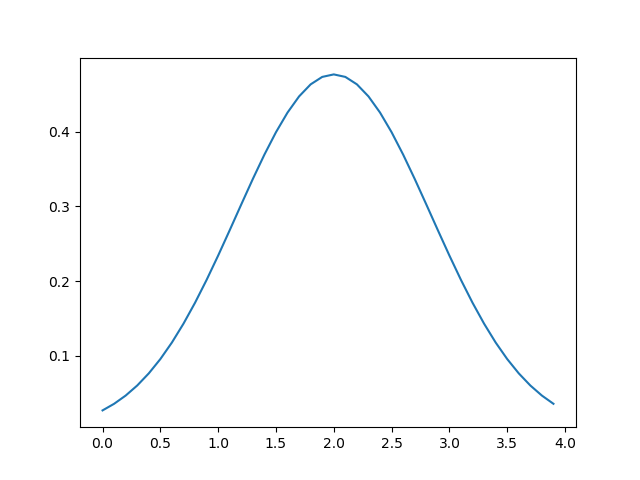
\includegraphics[width=0.4\textwidth]{kde1.png}
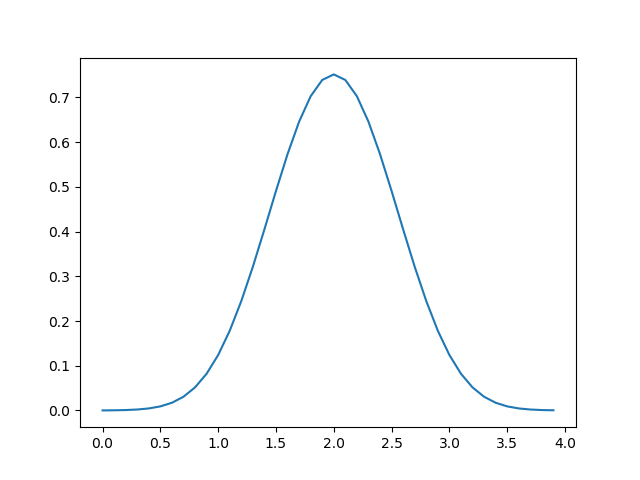
\includegraphics[width=0.4\textwidth]{kde2.png}
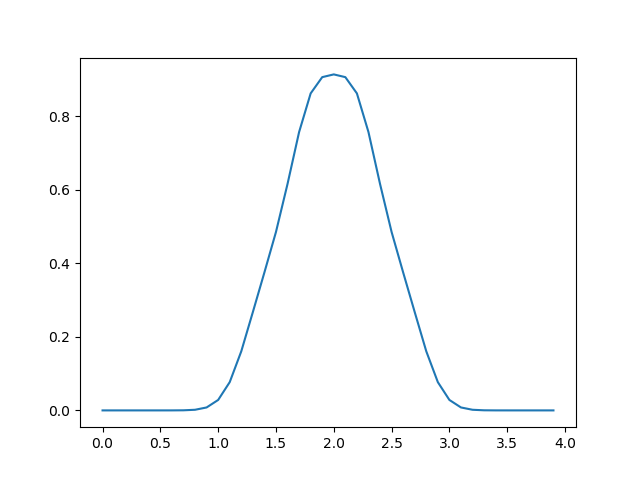
\includegraphics[width=0.4\textwidth]{kde3.png}
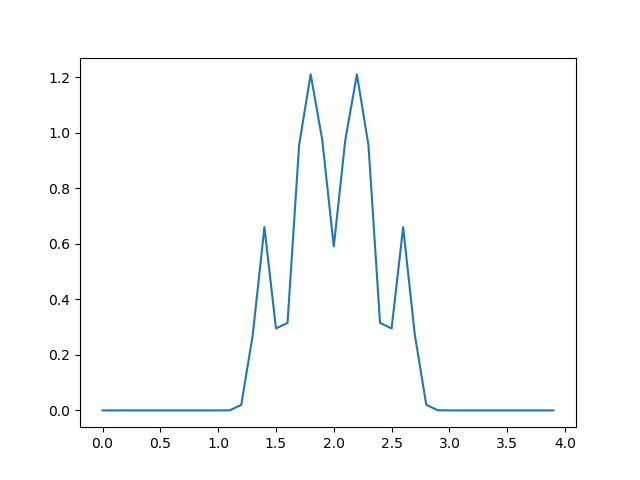
\includegraphics[width=0.4\textwidth]{kde4.png}
\caption{Gaussian KDEs with bandwidths of 2, 1, .5, and .2, respectively.}
\end{figure}

In practice, it's another parameter to play with. If the data follows a smooth
distribution, you can use a wider bandwidth which will ``blur" each data point
more and give a more intuitive view of the general distribution
characteristics. If the distribution is more ``wiggly," though, you need a
narrower bandwidth to see all the relevant detail.

Like most things in Data Science (and in life), there's no one true
hard-and-fast right answer. There is instead a range of points of view, many
of which may be illuminating.


